
The missing transverse energy is used to reject background events
where there is no natural source of missing energy, like in Drell-Yan and
QCD events. In the $\dytt$ process there is a large difference in the masses of 
$\tau$ and $\Z$. The taus are produced with large boost and their decay products, including 
neutrinos, are aligned with the leptons. Therefore a transverse component 
of missing energy with respect to the leptons is a better measure of true 
missing energy in the event, not originating from $\tau$ decay. 
To reject such background events with a small opening angle
between \met\ and one of the leptons, we used the projected \met~\cite{HWW2010} for 
event selection, defined as:
\begin{equation}
\text{with } \Delta\phi_{min} =  min(\Delta\phi(\ell_1,\met),\Delta\phi(\ell_2,\met))\\
\end{equation}
\begin{equation}
= 
\begin{cases} \met & \text{if $\Delta\phi_{min}>\frac{\pi}{2}$,}
\\
\met\sin(\Delta\phi_{min}) & \text{if $\Delta\phi_{min}<\frac{\pi}{2}$}
\end{cases}
\end{equation}
where $\Delta\phi(\ell_i,\met)$ is the angle between \met\ and lepton
 $i$ in the transverse plane.

In the presence of high multiple-interactions (pile-up), the instrumental \met\ tail in 
$\dyll$ events increases significantly. 
Figure~\ref{fig:met_pu} shows the projected particle-flow MET~\cite{PFMET} in the 
events with low ($<$5) and high ($>5$) primary vertices in both $\dyll$ data and MC. 
The $\dyll$ events in data are selected by requiring the dilepton invariant mass 
within 15 $\GeVcc$ of the $Z$ mass. 
%
%Commented out this figure AY
%
%This leads to a large increase of the background contribution in the signal region, as shown in 
%Figure~\ref{fig:meteff_pu}. 
%
%This causes a sharp increase in the efficiency for $\dyll$ events to pass a given \met\ 
%requirement as the number of pile-up interactions increases. 
%To improve the robustness of the \met\ performance in the presence of pile-up, 
To improve the signal over background performance of \met\ selections in the presence of pile-up, 
we have developed a novel \met\ algorithm referred to as ``trk-MET''~\cite{trkMET}, constructed from 
charged particles consistent with originating from the primary vertex. 
The event $\met$ trk-MET is defined as 
\begin{equation}
\text{trk-MET} \equiv -\overrightarrow{p_T}(l_1) - \overrightarrow{p_T}(l_2) - \sum_i{\overrightarrow{p_T}(i)}, \\
\label{eq:trkmet}
\end{equation}
where $\overrightarrow{p_T}(l_1)$ and $\overrightarrow{p_T}(l_2)$ are the transverse momentum vectors of the two 
leptons passing the lepton selections described in Sec.~\ref{sec:sel_muons} and Sec.~\ref{sec:sel_electrons}, 
and $\overrightarrow{p_T}(i)$ represent the tranverse momentum vectors of the charged PFCandidates satisfying the following requirements:
%%%%%%%%%%%%%%%%%%%%%%%%%%
\begin{itemize}
\item the track matched to PFCandidate has $\Delta z < 0.1$~cm with respect to the signal PV, which is the 
closest PV to the track in $\Delta z$;
\item the track has $\Delta R > 0.1$ with respect to both leptons, to avoid double-counting of the leptons.
\end{itemize}
%%%%%%%%%%%%%%%%%%%%%%%%%%

Comparing to the projected PFMet, we observed that the projected trk-MET has 
a larger tail in $\dyll$ background events~\cite{trkMET}. 
However these two \met\ values are weakly-correlated in $\dyll$ backgrounds with no geninue $\met$, and 
strongly correlated for the signal processes with geninue $\met$, as shown in Figure~\ref{fig:met_scatter}. 
Therefore the signal over background ratio is improved if we select the events 
based on the mininum of these two projected $\met$ values, $\text{min-MET} \equiv min(\text{proj}_\text{trk-MET}, \text{proj}_\text{PFMET})$. 


The selection requirements are different between \ee{}/\mm{}
and \emu{} final states since Drell-Yan mostly contributes to \ee\
and \mm\ channels. The selection requirements are:
\begin{itemize}
\item min-MET $>20~\GeV$ for \emu{}
\item min-MET $>35~\GeV$ for \ee{} and \mm{} 
\end{itemize}
The selection efficiencies for the signal ($\hww$ at $m_{H}=130$ GeV) and background ($\dyll$) 
events are shown in Figure~\ref{fig:met_eff} as a function of $\met$ requirements. 
Using min-MET we see that the signal selection efficiency improves while the background selection efficiency reduces significantly 
compared to the values obtained using projected PFMet. 
In addition, the background selection efficiency dependendence on the 
number of primary vertices is largely reduced as well using min-MET. 


%%%%%%%%%%%%%%%%%%%%%%%%%%%%%%%%%%%%%%%%%%%
\begin{figure}[hbt]
\begin{center}
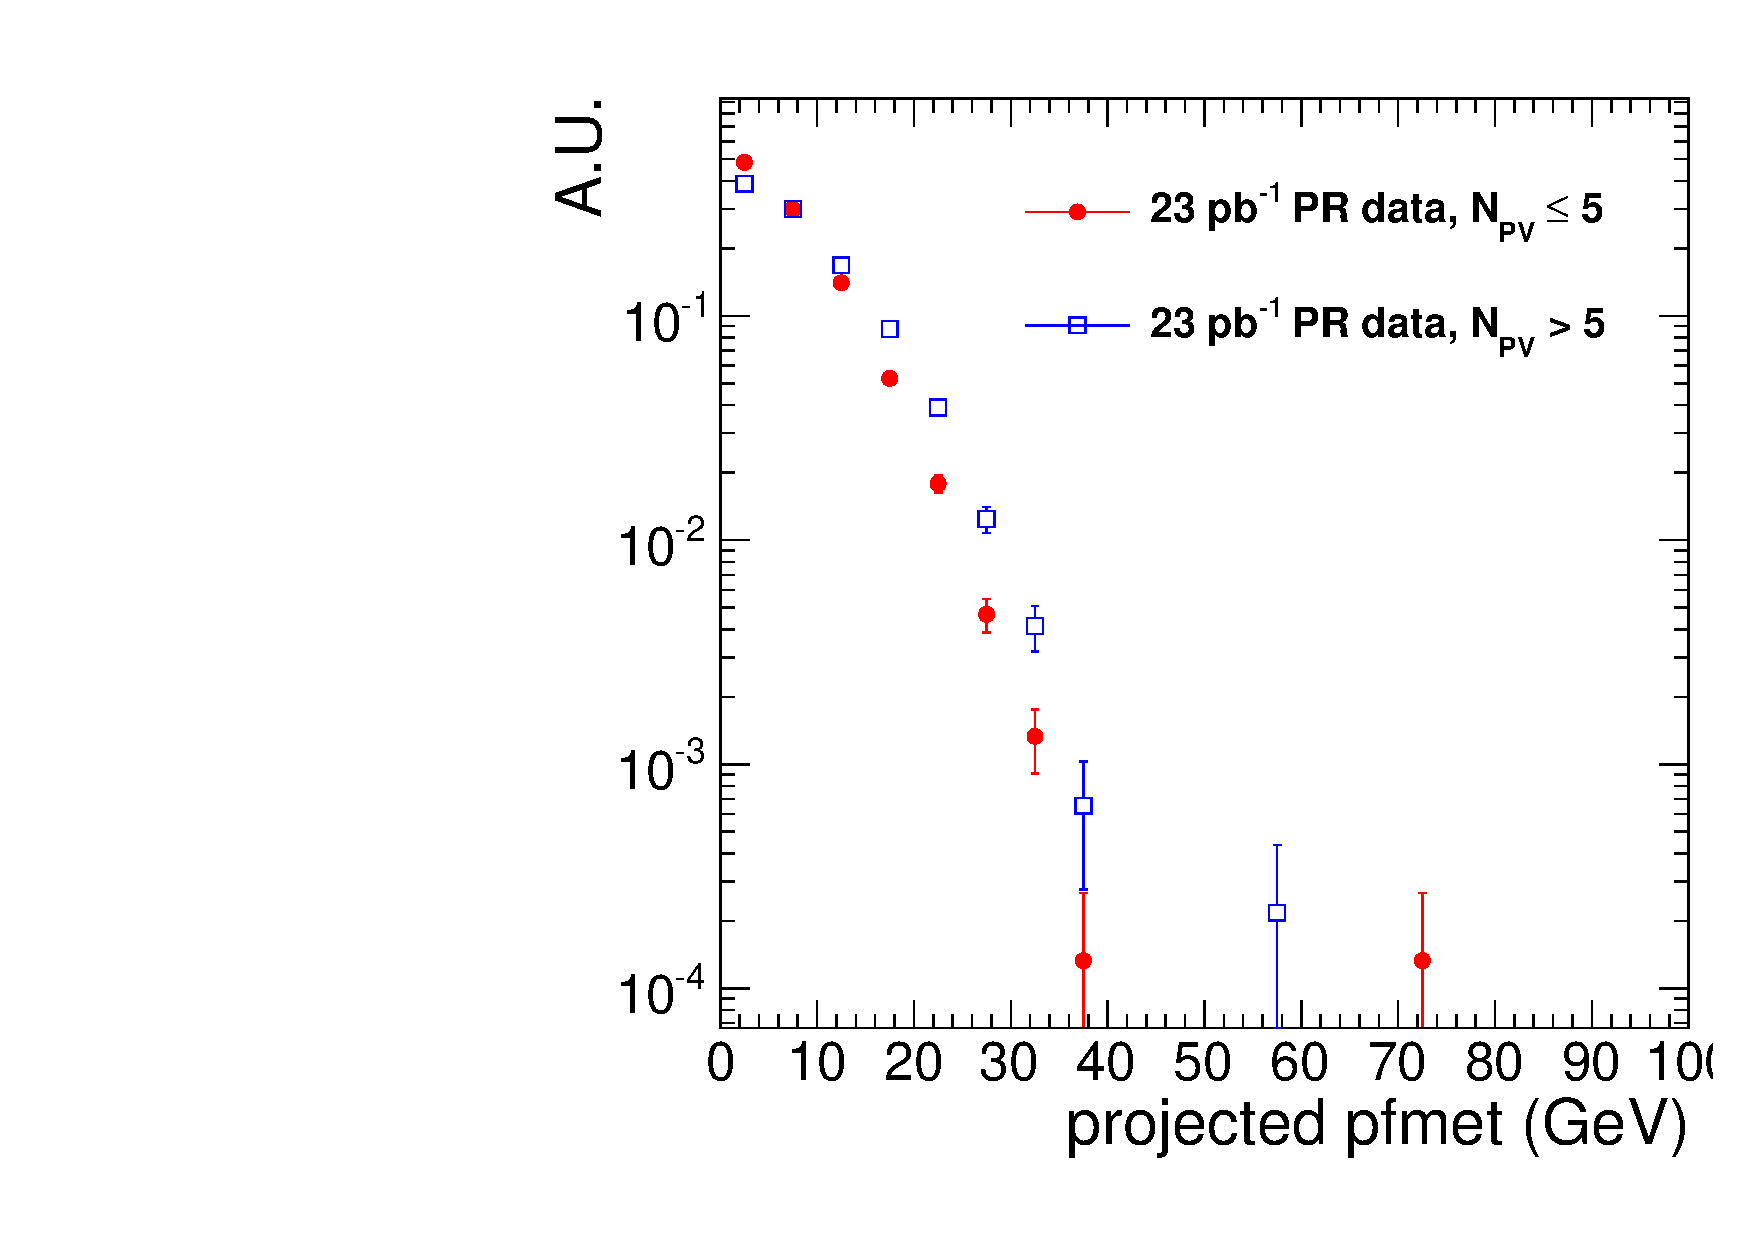
\includegraphics[width=0.4\linewidth]{figures/pfmet_data.pdf} 
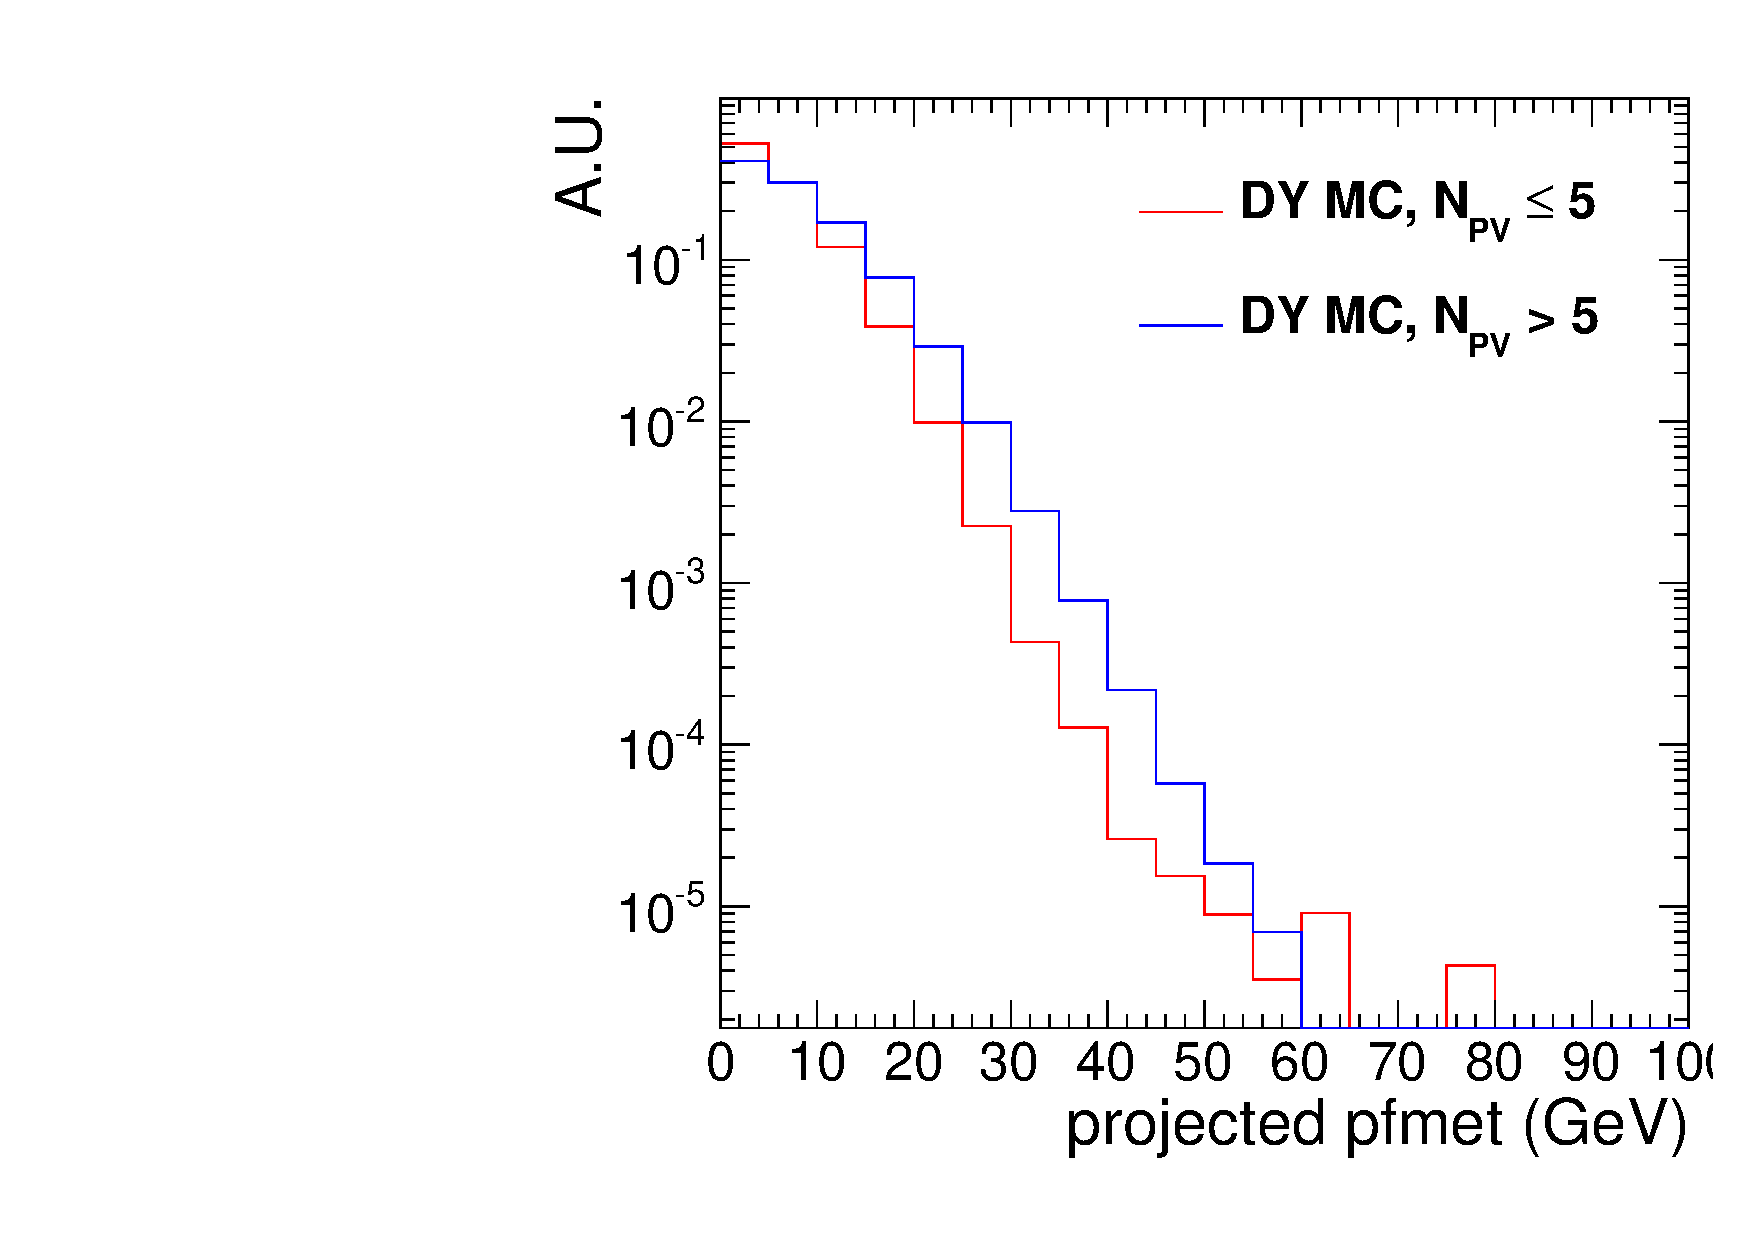
\includegraphics[width=0.4\linewidth]{figures/pfmet_dymc.pdf}
%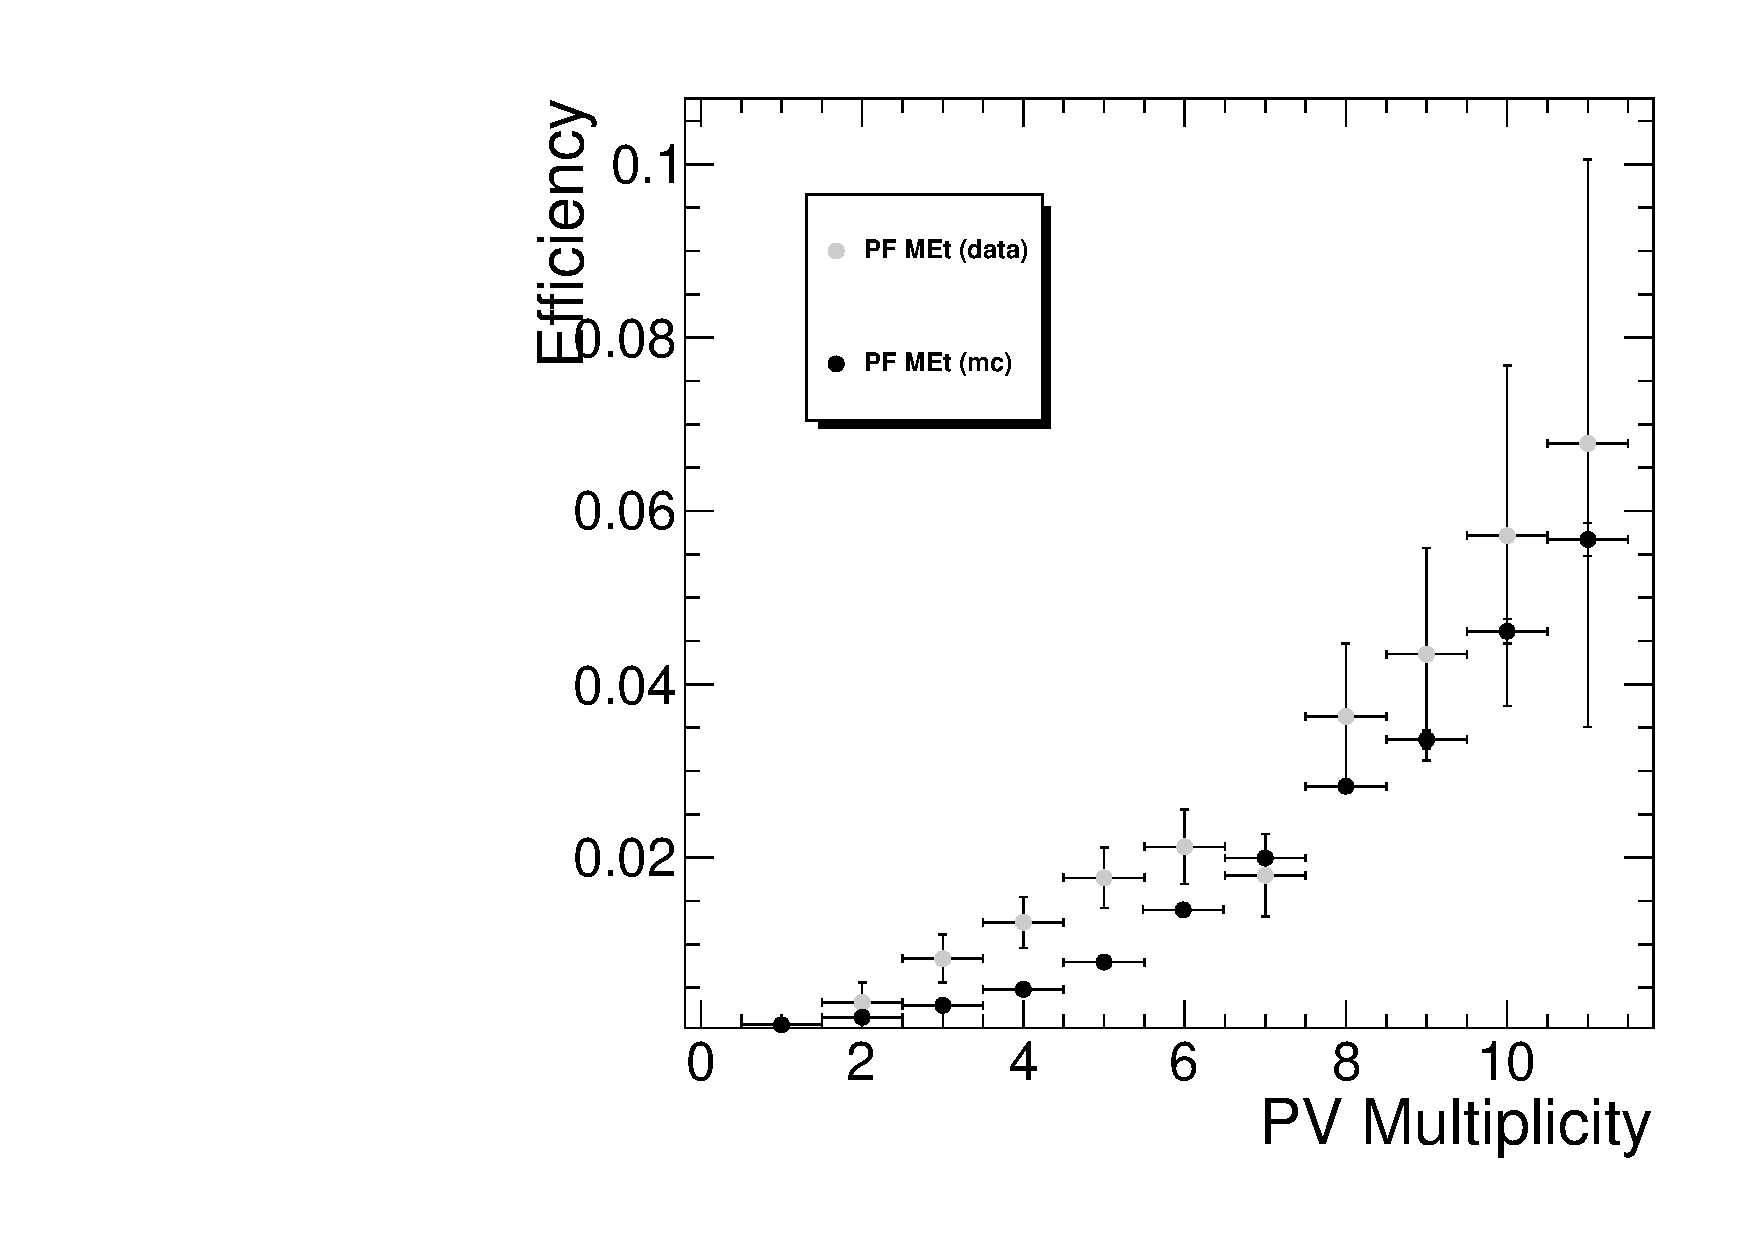
\includegraphics[width=0.3\linewidth]{figures/pfmet_Eff30.pdf} 
\caption{\label{fig:met_pu}\protect Distributions of projected PFMet in data (left) and $\dyll$ MC (center) 
overlayed for low pile-up and high pile-up.}
\end{center}
\end{figure}
%%%%%%%%%%%%%%%%%%%%%%%%%%%%%%%%%%%%%%%%%%%
%%%%%%%%%%%%%%%%%%%%%%%%%%%%%%%%%%%%%%%%%%%

%%
%%% figure makes no sense, commented out AY
%%
%\begin{figure}[hbt]
%\begin{center}
%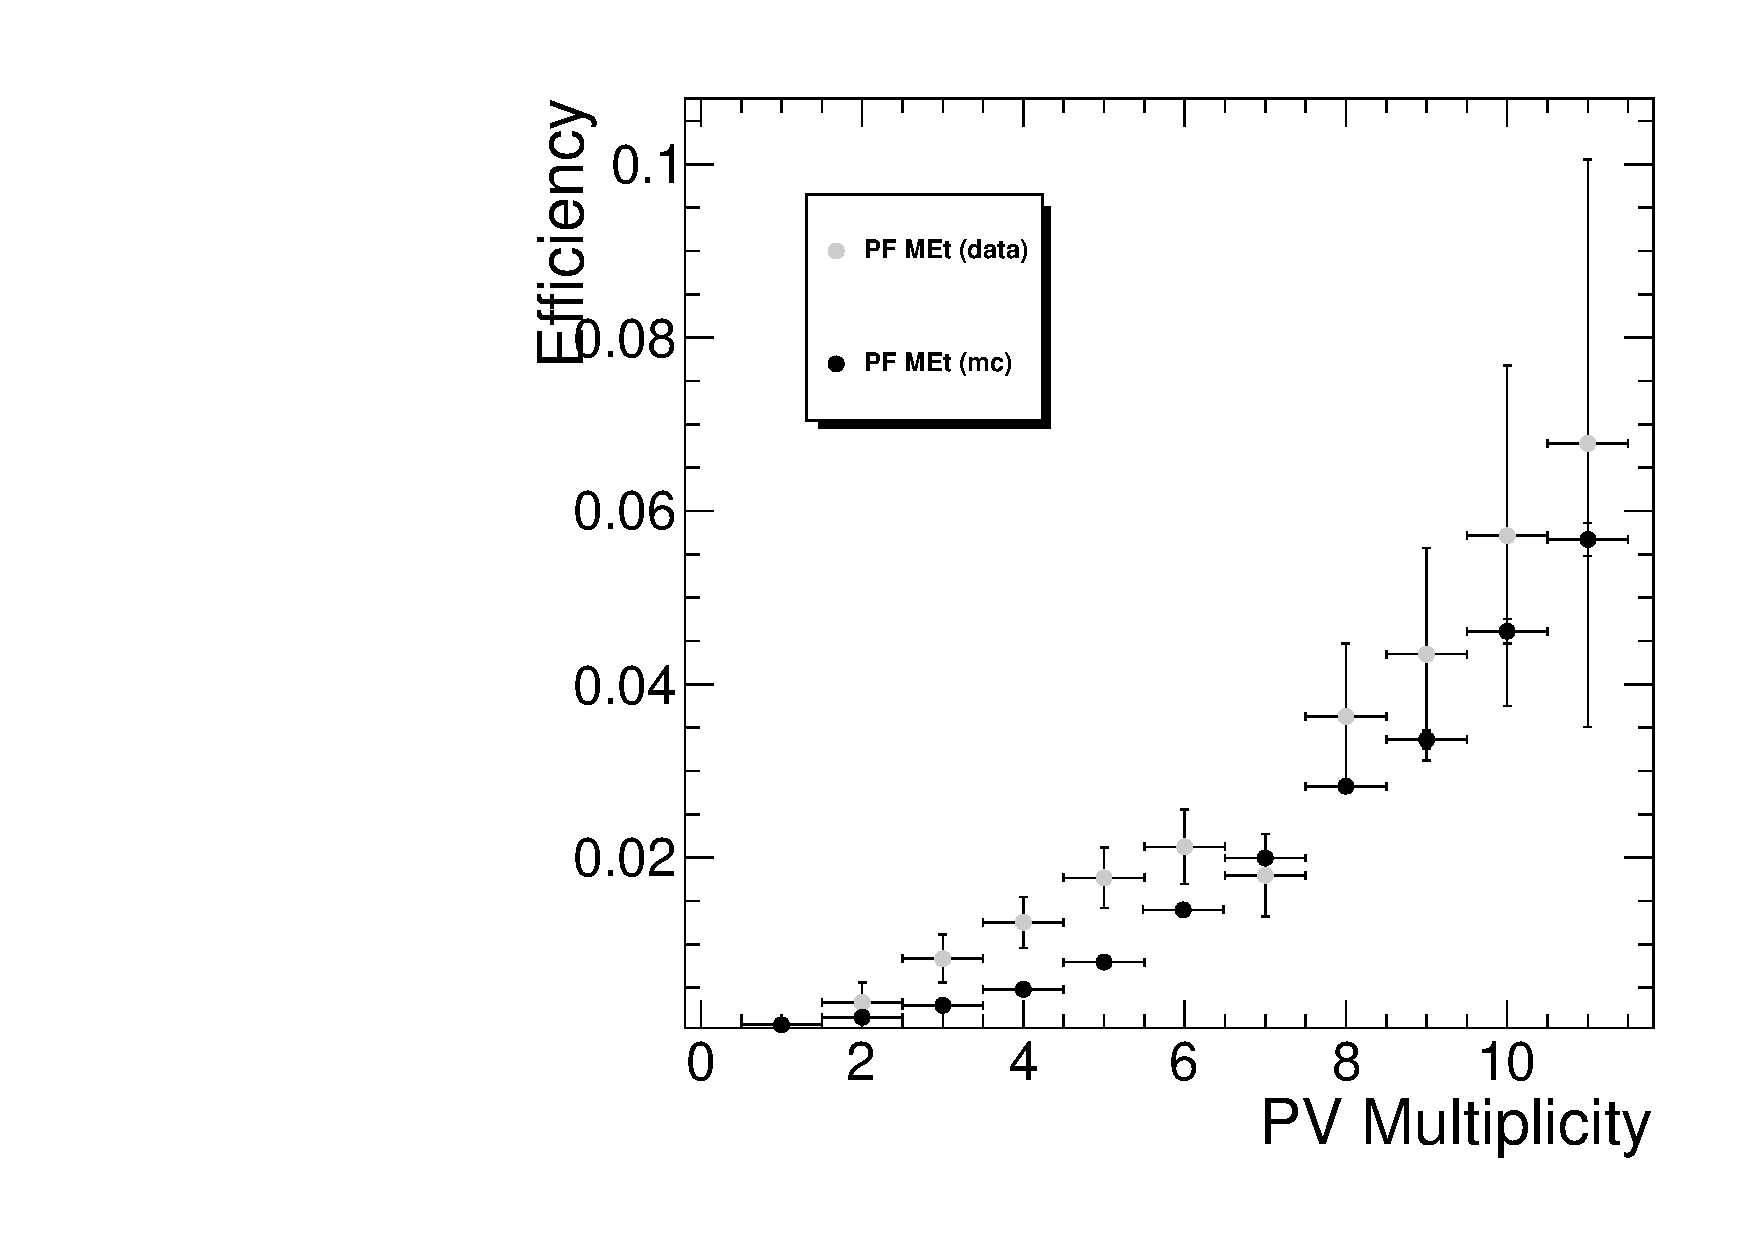
\includegraphics[width=0.5\linewidth]{figures/pfmet_Eff30.pdf} 
%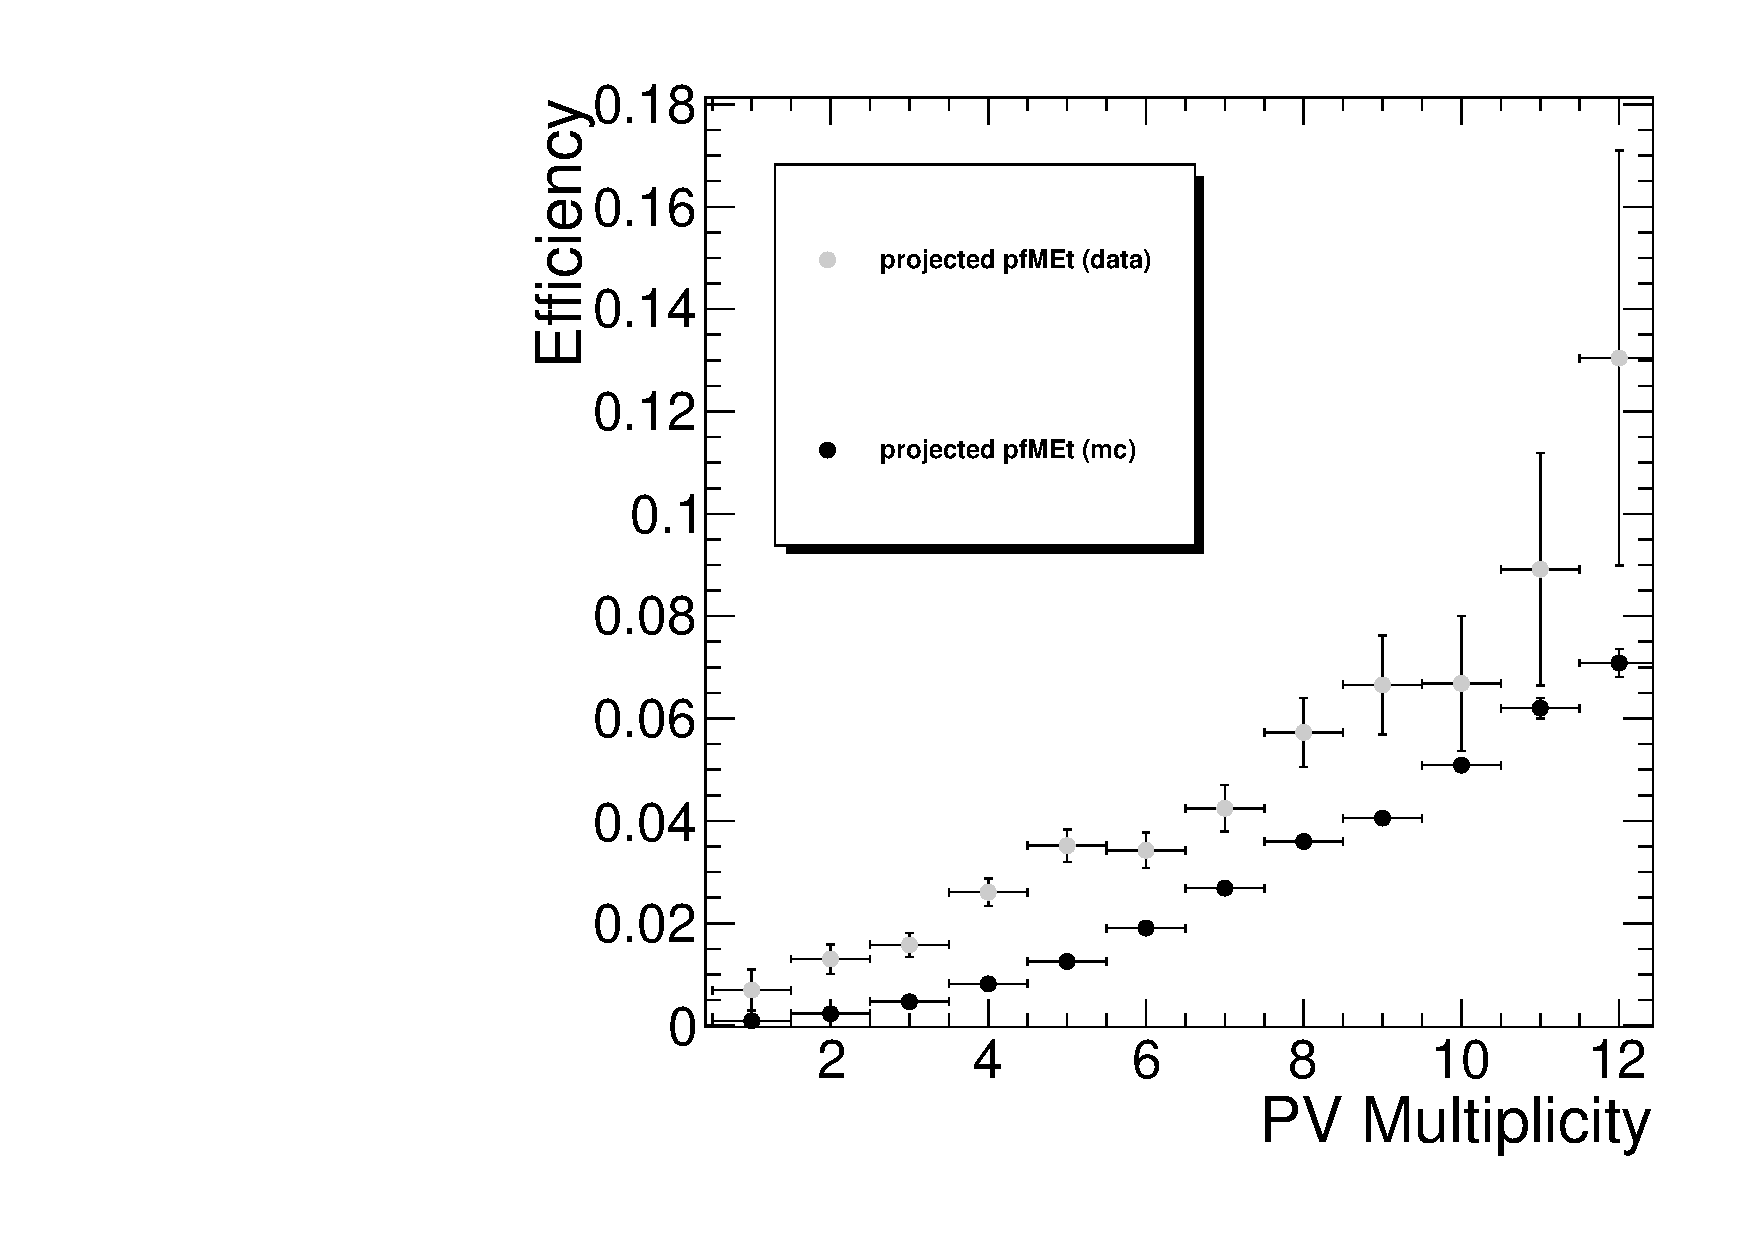
\includegraphics[width=0.5\linewidth]{figures/proj_pfmet_Eff25.pdf} 
%\caption{\label{fig:meteff_pu}\protect The efficiency to satisfy the requirement projected pfmet$>25$~GeV as a %function
%of the number of reconstructed vertices in $\dyll$ data and MC.}
%\end{center}
%\end{figure}
%%%%%%%%%%%%%%%%%%%%%%%%%%%%%%%%%%%%%%%%%%%

%%%%%%%%%%%%%%%%%%%%%%%%%%%%%%%%%%%%%%%%%%%
\begin{figure}[hbt]
\begin{center}
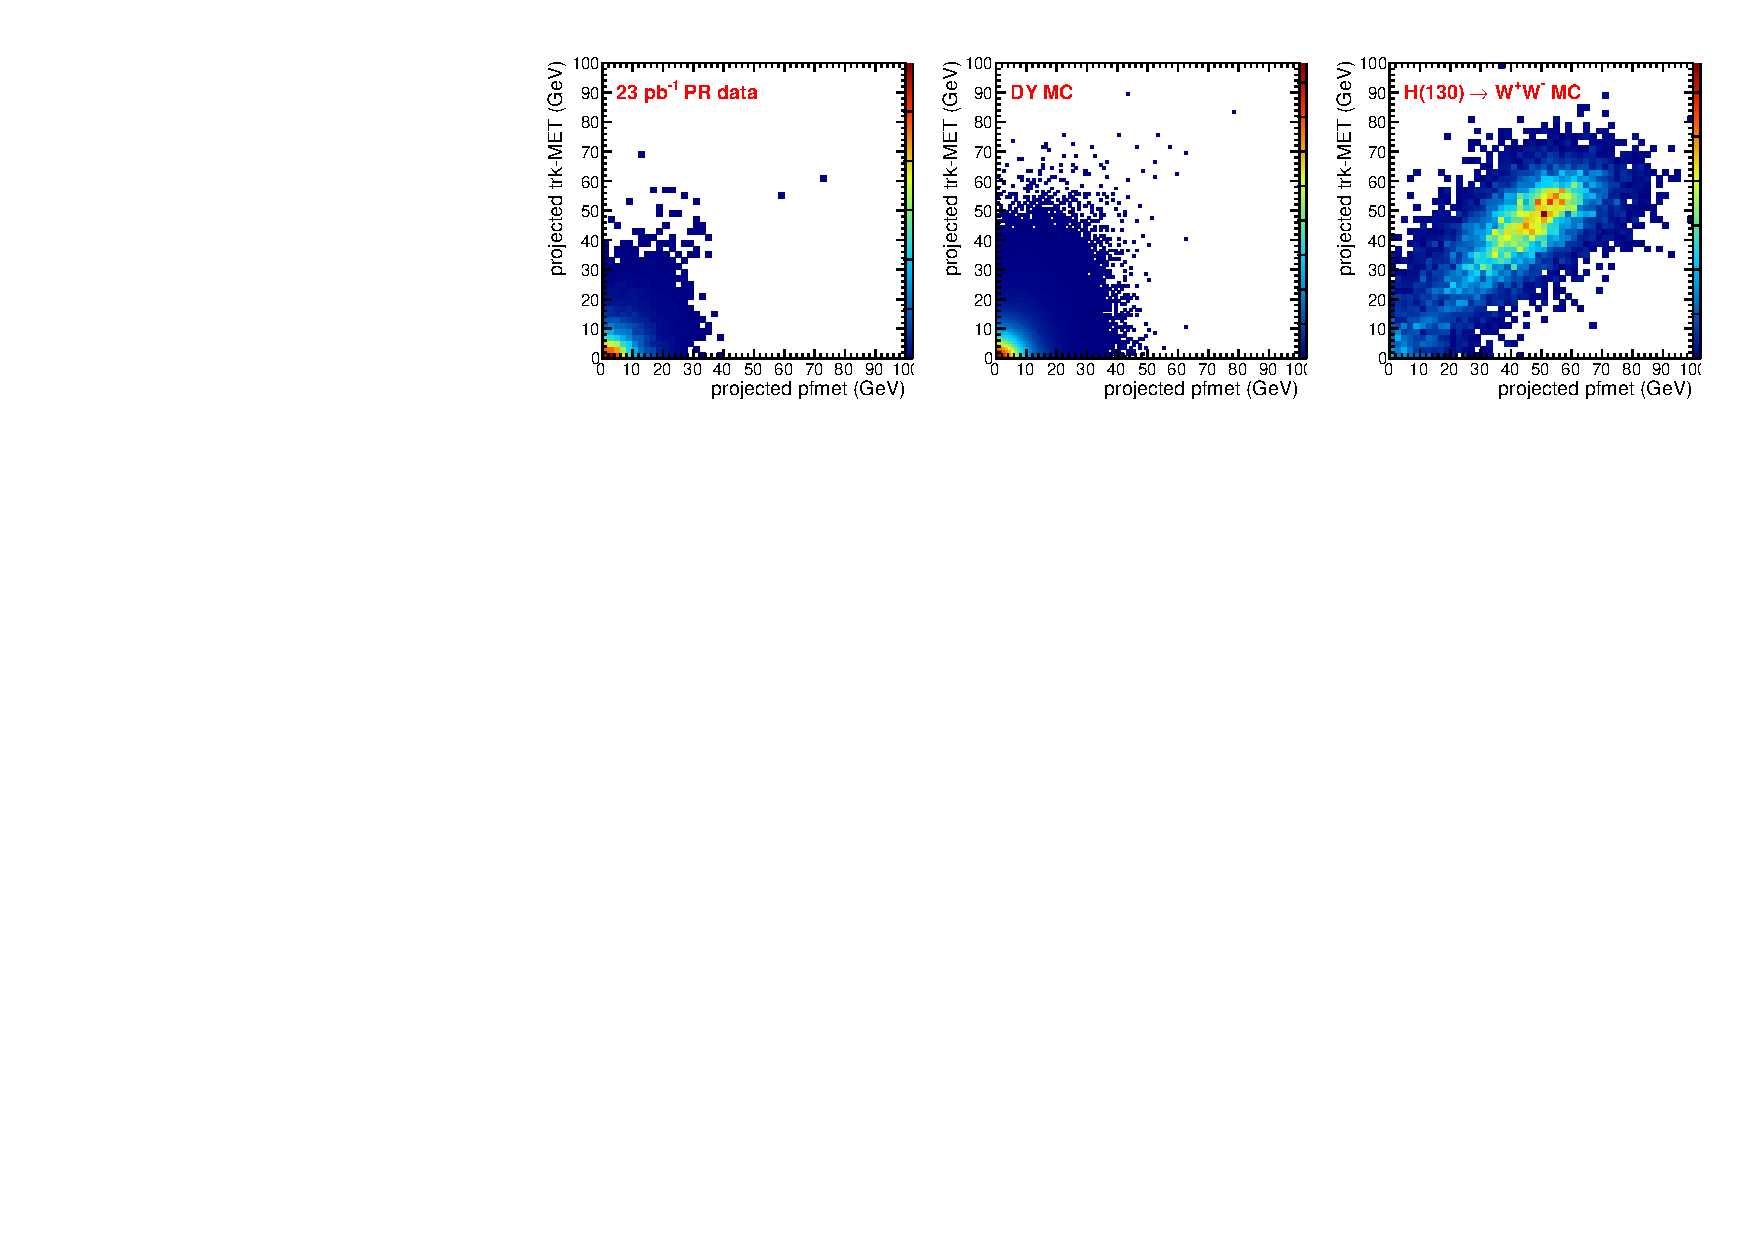
\includegraphics[width=1\linewidth]{figures/met_scatter.pdf} 
\caption{\label{fig:met_scatter}\protect Distributions of trk-MET vs. pfmet in data (left), $\dyll$ MC (center) and Higgs MC (right).}
\end{center}
\end{figure}
%%%%%%%%%%%%%%%%%%%%%%%%%%%%%%%%%%%%%%%%%%%

%%%%%%%%%%%%%%%%%%%%%%%%%%%%%%%%%%%%%%%%%%% 
\begin{figure}[hbt]
\begin{center}
%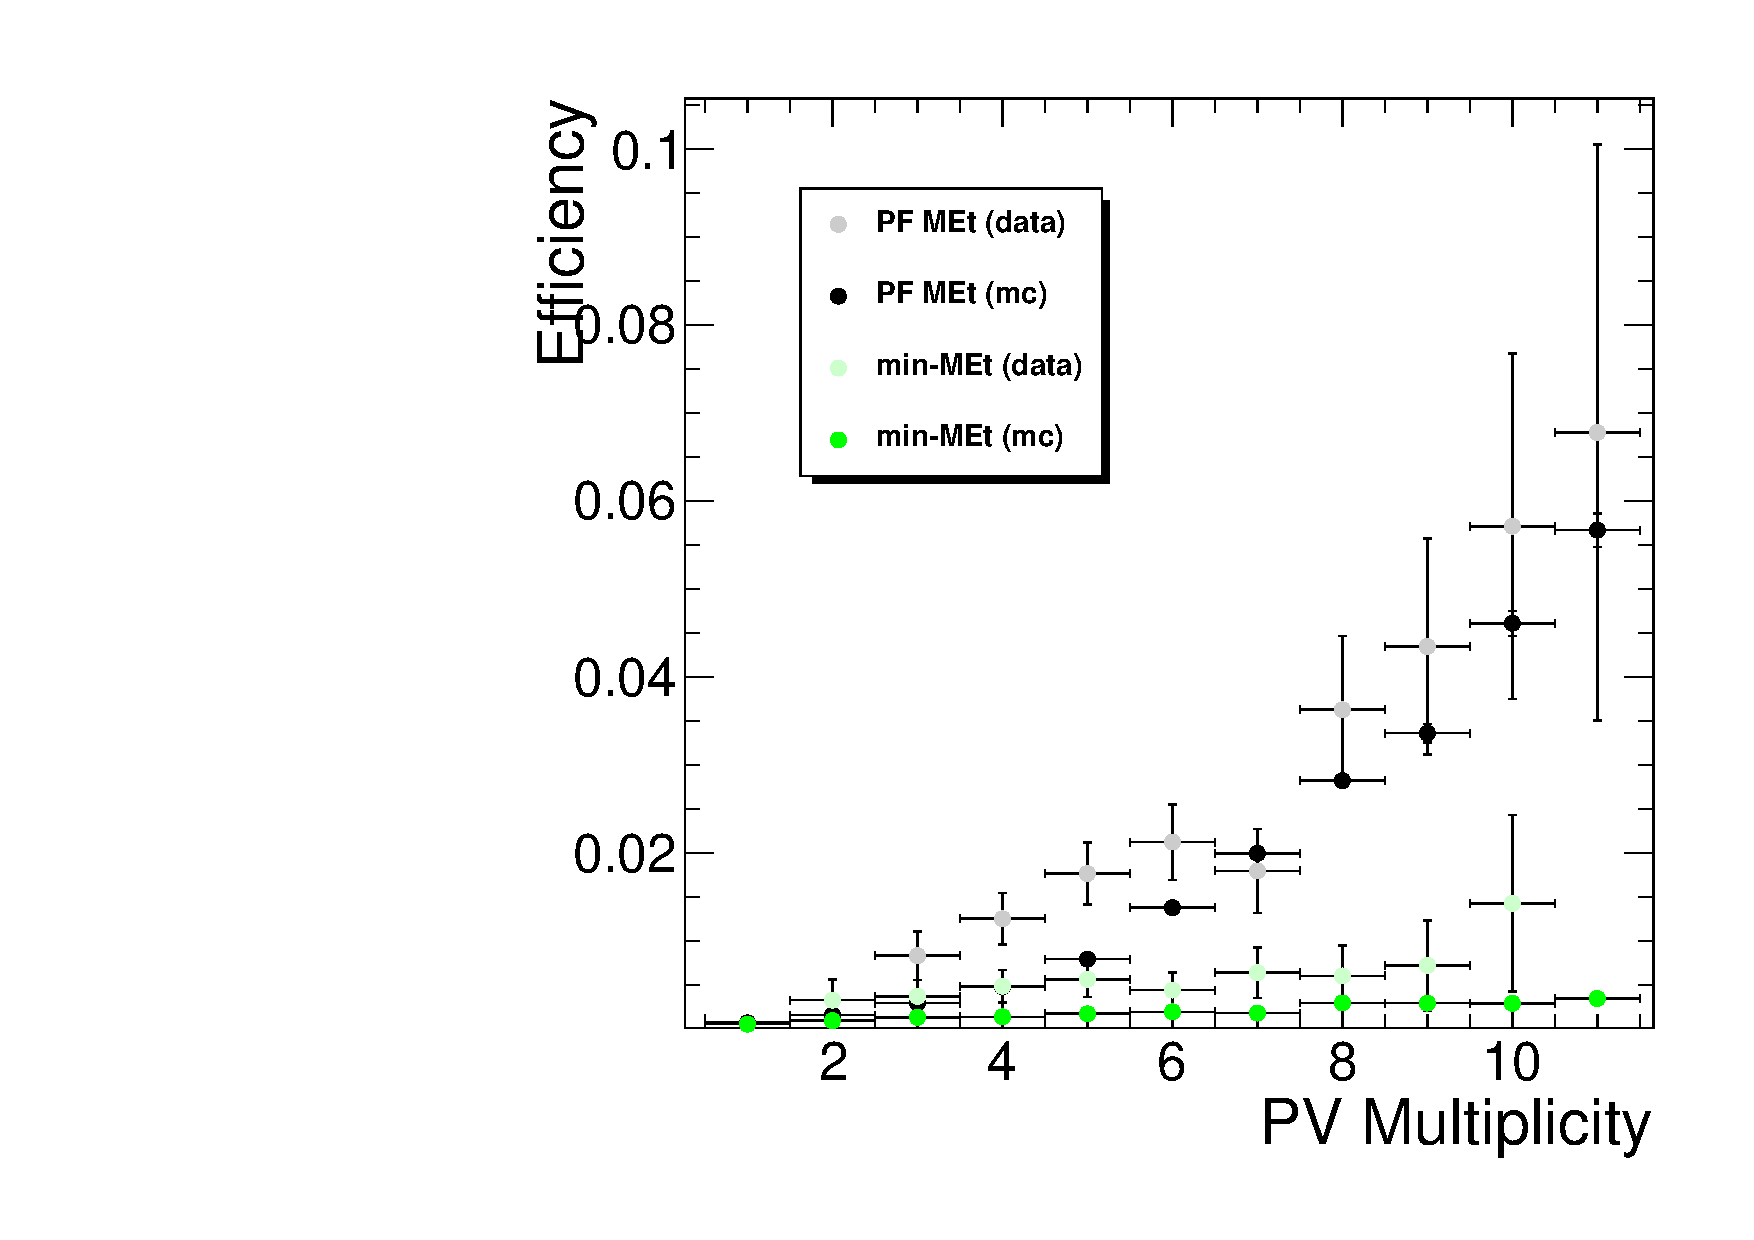
\includegraphics[width=0.45\linewidth]{figures/pfmet_minmet_Eff30.pdf} 
%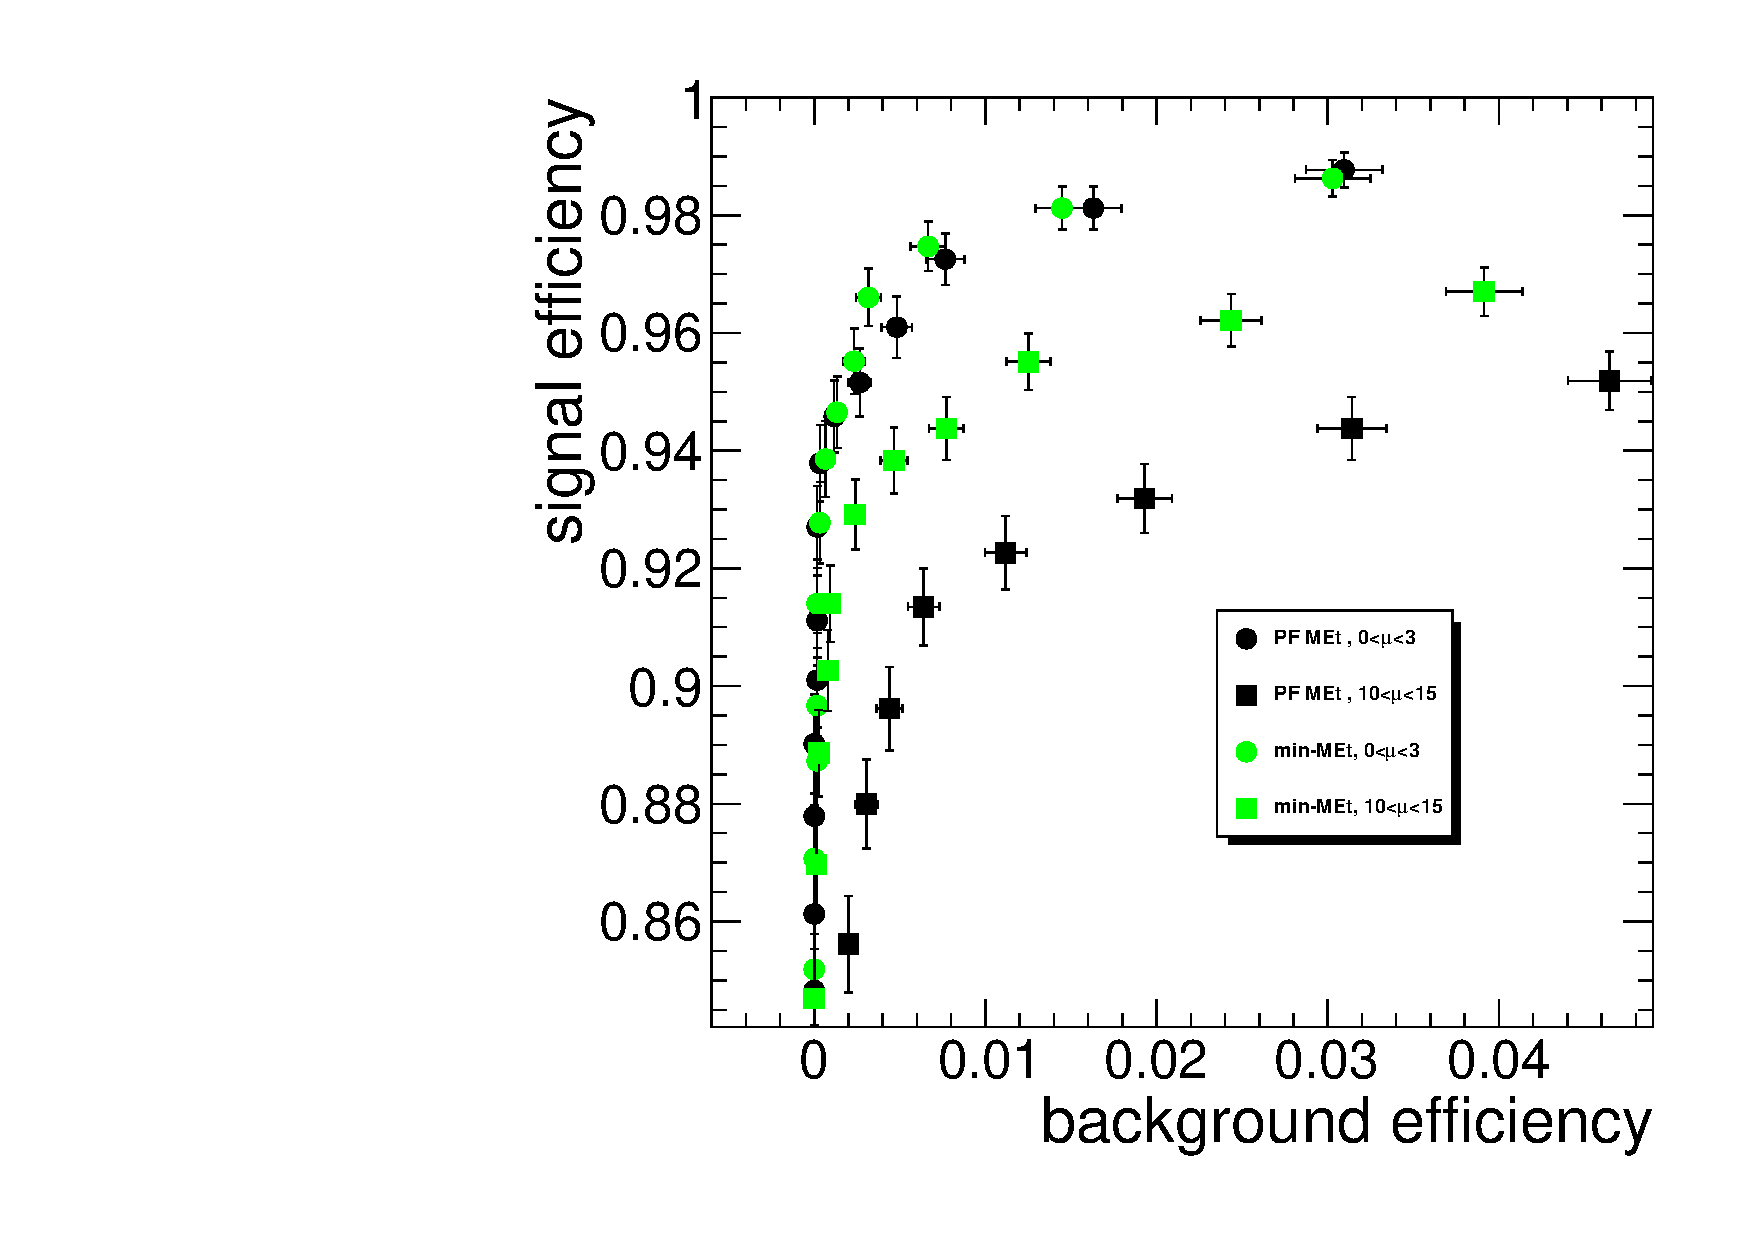
\includegraphics[width=0.45\linewidth]{figures/SignalVsBkgrEfficiency.pdf} 
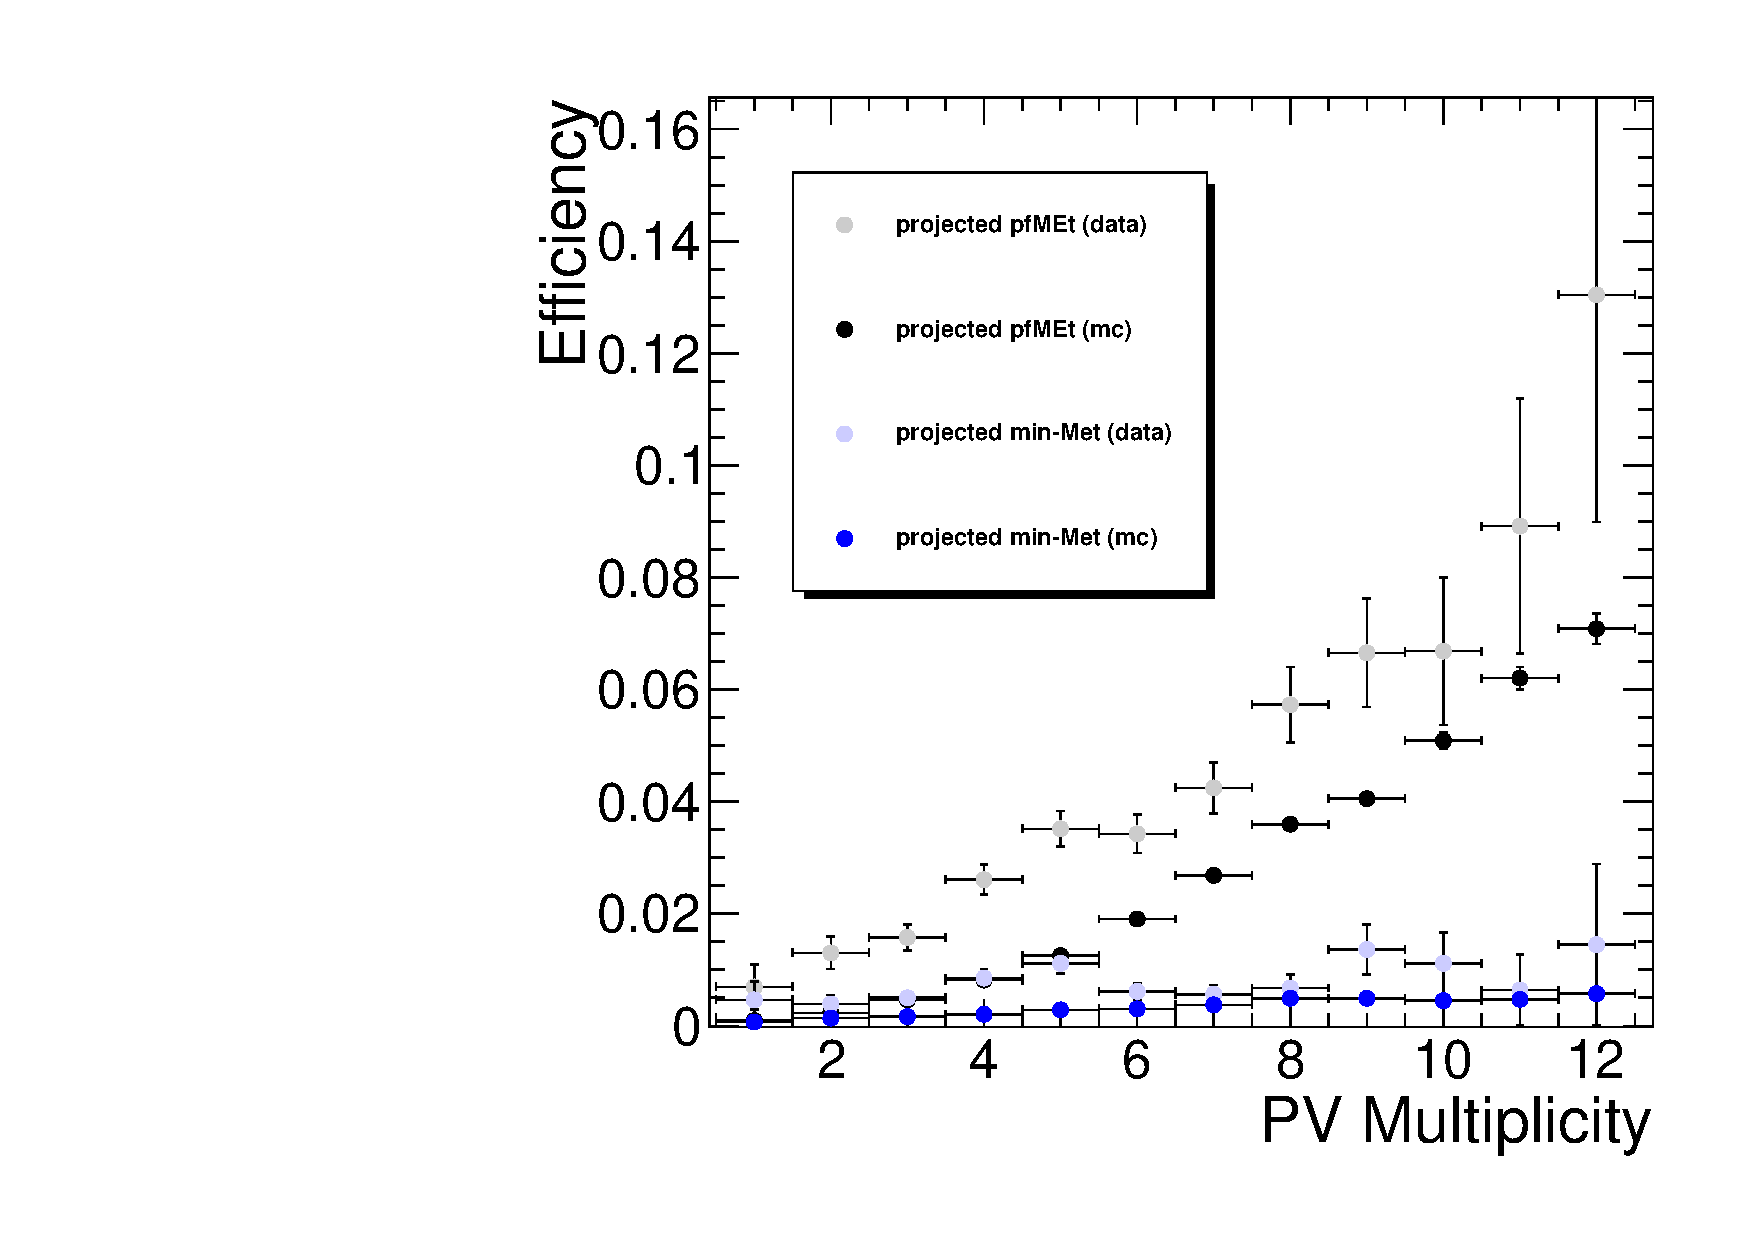
\includegraphics[width=0.45\linewidth]{figures/proj_pfmet_minmet_Eff25.pdf} 
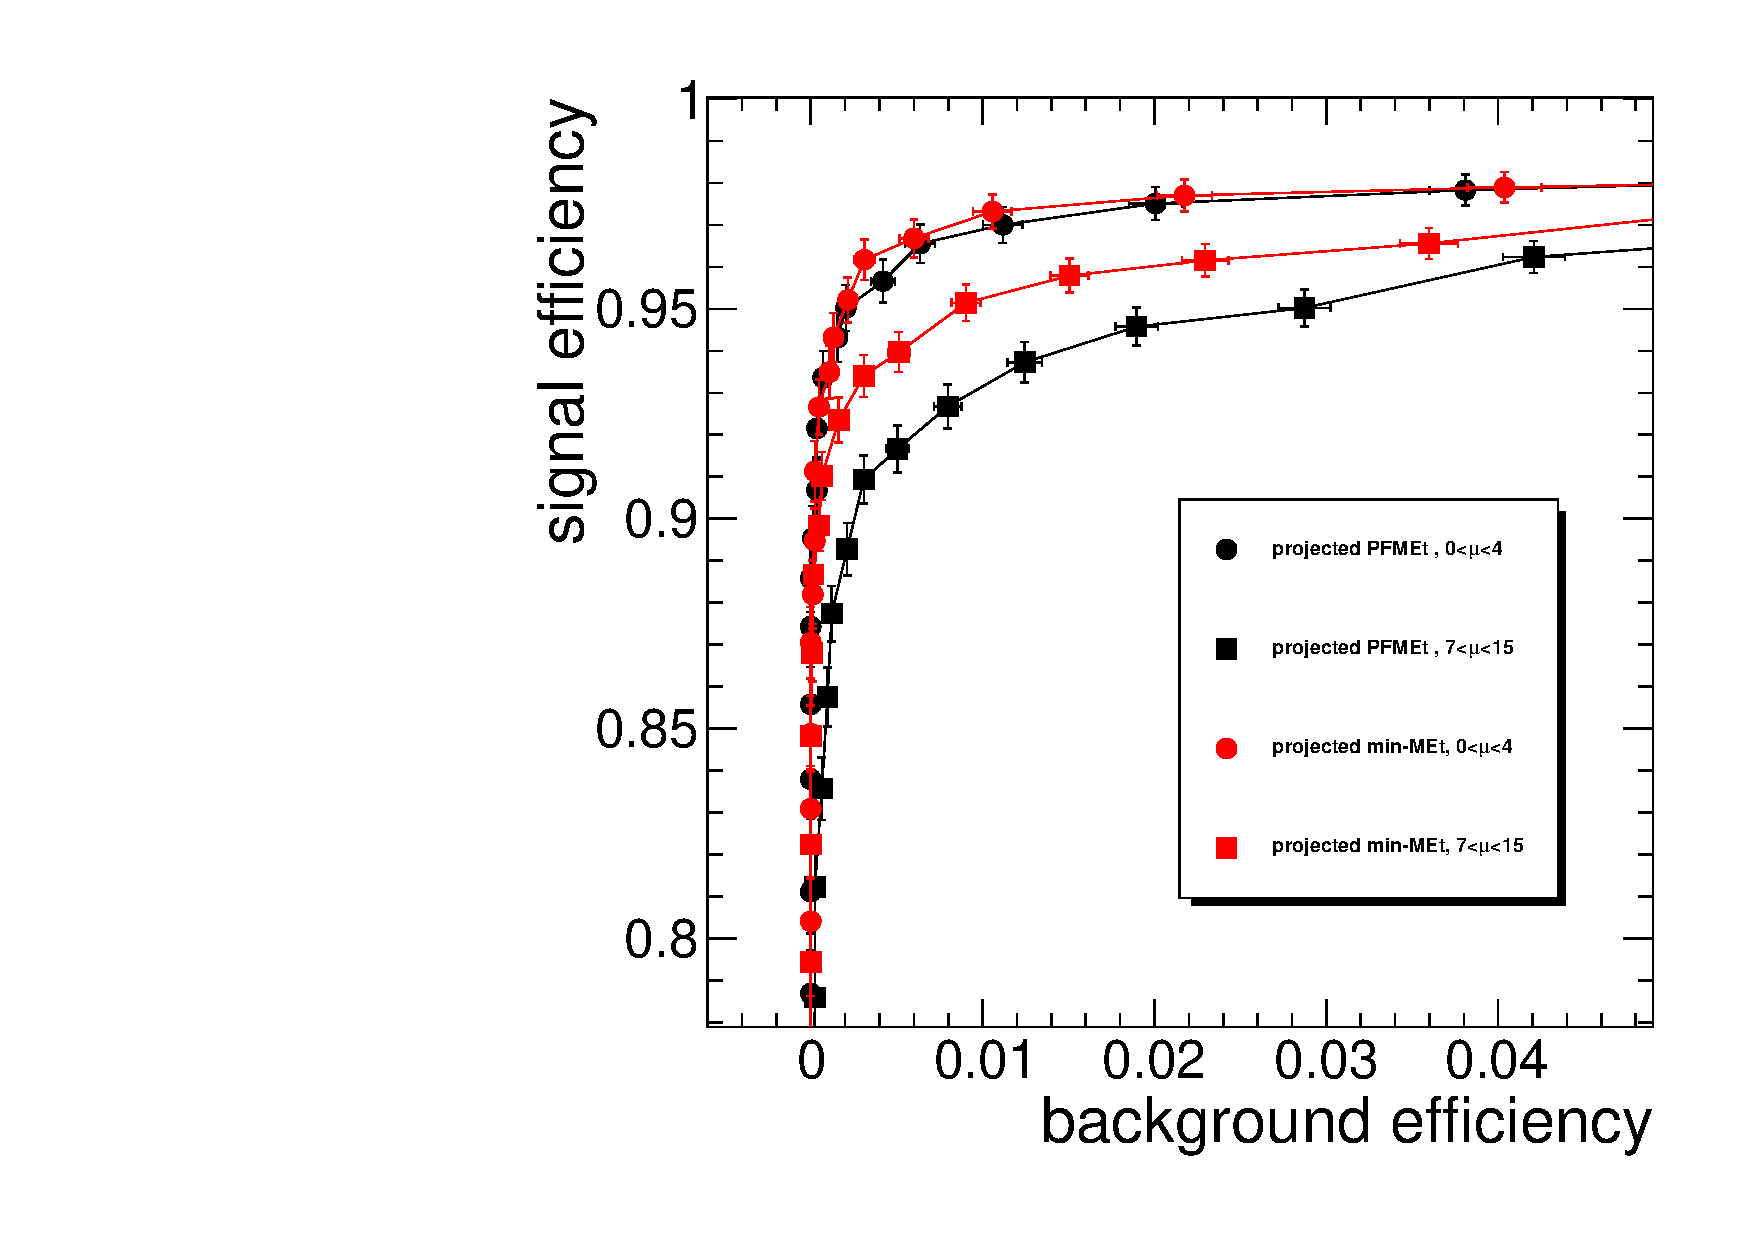
\includegraphics[width=0.45\linewidth]{figures/pMetSignalVsBkgrEfficiency.pdf} 
\caption{\label{fig:met_eff}\protect Left plot shows the efficiency to satisfy
 the requirement projected (pf or min) met$>25$~GeV as a function of the number of reconstructed 
vertices for Z-events in data and MC. Right plot shows the signal efficiency 
vs. background efficiency, evaluated for H$_{160}$ and $\dyll$ MC.}
\end{center}
\end{figure}
%%%%%%%%%%%%%%%%%%%%%%%%%%%%%%%%%%%%%%%%%%%



%In the presence of high pile-up, the instrumental \met\ tail in $\dyll$ events is enhanced
%significantly, as shown in Figure~\ref{fig:met_pu} for data and $\dyll$ MC. This causes a sharp increase in the
%efficiency for $\dyll$ events to pass a given \met\ requirement as the number of pile-up
%interactions increases. To improve the robustness of the \met\ performance
%in the presence of pile-up, we have developed a novel \met\ algorithm (trk-MET).
%trk-MET is \met\ constructed from charged particles consistent with originating from
%the signal PV. We correct for the 2 leptons, as well as charged PFCandidates which satisfy
%the following requirements:
%\begin{itemize}
%\item the track matched to PFCandidate has $\Delta z < 0.1$~cm with respect to the signal PV;
%\item the signal PV is the closest PV to the track in $\Delta z$;
%\item the track has $\Delta R > 0.1$ with respect to both leptons, to avoid 
%double-counting of the leptons.
%\end{itemize}
%The high \met\ tail in events with no genuine \met\ is larger for trk-MET than for pfmet. However,
%we observe that for data and MC $\dyll$ events these two \met\ flavors are weakly-correlated, as shown
%in Figure~\ref{fig:met_scatter}. Therefore the rejection power for $\dyll$ events is increased significantly
%by cutting on both pfmet and trk-MET, or equivalently by cutting on min-MET $\equiv$ minimum(pfmet,trk-MET).
%In addition, the high \met\ tail efficiency vs. number of pile-up interactions is flattened, as shown
%in Figure~\ref{fig:met_eff}. For signals with genuine \met\, trk-MET and pfmet are strongly correlated. 
%The signal (H(130) MC) efficiency vs. background ($\dyll$ MC) efficiency is shown in 
%Figure~\ref{fig:met_eff} for min-MET and pfmet.
